\section{Desagregação de chuvas}

O método de desagregação de chuvas trata-se de uma metodologia com vantagem de uso simples, fornecendo resultados satisfatórios e com boa similaridade para locais distintos, além de permitir uma validade para regiões próximas onde não há medição. (TORICO, 1975) desenvolveu a metodologia das isozonas, que pode ser aplicada em todo o território nacional. Dentro dos métodos mais utilizados, destacam-se os trabalhos de (DAMÉ, 2006) e Damé et al (2003), onde foi utilizado séries de chuvas sintéticas para estimar as correlações de intensidade-duração-frequência, porém a metodologia mais utilizada está naquela que correlaciona a duração de chuvas com maiores durações para chuvas intensas de durações inferiores.

O método das isozonas foi comparado, pelos órgãos responsáveis pelas rodovias do Estado de Goiás e Departamento Nacional de Estradas e Rodagem, com as equações de chuvas intensas e encontraram desvios entre 7,0 e 55\%, sendo recomendada a busca por outra metodologia de cálculo Costa e Rodrigues (1999).

O método de desagregação de chuvas pode ser encontrado na literatura diversas metodologias para obter durações de chuvas intensas de menores durações a partir de uma chuva de maior duração.

\begin{figure}
    \caption{Representação da desagregação de chuvas}
    \centering
    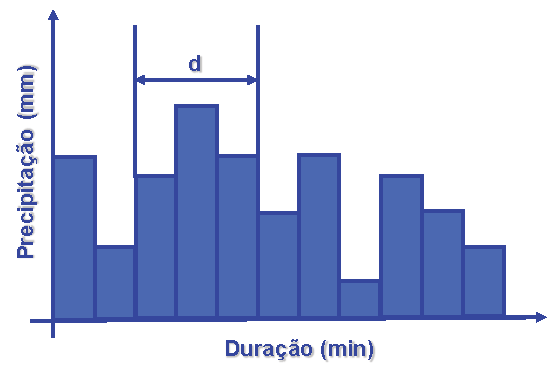
\includegraphics[width=0.7\textwidth]{Textuais/Figuras/desagregacao.pdf}
    \fonte{Autores}
    \label{fig:desagregacao}
\end{figure}

\subsection{Damé (2001)}

Para Damé (2001) foram utilizados os parâmetros do modelo Bartlett-Lewis do Pulso Retangular Modificado (BLPRM) (Rodriguez-Iturbe, 1987) e, como consequência, as séries de chuvas na duração de 15 minutos foram separadas de uma chuva com duração de 24 horas e implementadas no modelo de desagregação proposto por Glasbey et al (1995).

O modelo BLPRM considera como hipótese que a precipitação tenha estacionalidade mensal, ou seja, que suas propriedades estatísticas (média, variância, covariância, probabilidade de ocorrência de períodos secos) não se alterem dentro do mês. No trabalho de Damé et al (2003) o método das relações (MR) foi utilizado para obter uma curva IDF histórica obtida por meio de dados pluviográficos para o mesmo período de anos; os resultados mostram que a IDF obtida pelo MR representou adequadamente a IDF histórica, levando os autores concluírem que este método é eficaz na desagregação da chuva diária. Dessa forma, é viável a possibilidade de usar esse método para obter relações de intensidade-duração-frequência em regiões nas quais se tenha pouco ou nenhuma informação pluviográfica e que existam abundantes registros de chuva diária.

Assumindo de que o método das relações foi eficaz na separação de chuvas diárias e que forneceu resultados próximos aos que seriam obtidos por meio do uso de plataforma de coleta de dados, verificou-se o desempenho das estimativas dos valores de intensidades máximas, quando se utiliza o método das relações para desagregar a chuva diária e estimar as relações IDF e assim chegar a uma conclusão sobre o método das relações.

\subsection{Bell (1969)}

De acordo com Bell (1969) estabeleceu relações experimentais entre chuvas com diferentes durações fundamentado em informações de séries fracionais de chuva observada nos EUA, Austrália, URSS, Porto Rico, Alasca, África do Sul e Havaí. O fundamento teórico desse estudo é a existência de similaridade entre a formação de chuvas. Devido a propriedades semelhantes em muitas partes do mundo devido a características de chuvas convectivas,  utiliza-se a equação de Bell para estimar a chuvas máximas entre os limites especificados. Devido a esse estudo ter sido realizado em diversas partes do mundo o trabalho de Bell apresenta algumas limitações. Devido aos valores adotados serem de várias regiões do mundo esses valores representam valores médios e não específicos de uma região; um outra limitação está na durações das chuvas, que devem estar entre 5 minutos e 120 minutos; pode- se, também destacar, como limitação ao método de Bell, a obrigatoriedade de se conhecer a precipitação máxima com duração de 60 minutos e intervalo de retorno de 10 anos, sendo necessário a coleta de dados por meio de pluviógrafos.

Bell (1969) utilizou dados de vários continentes e ajustou a Equação 8.

\subsection{Chen (1983)}

Chen (1983) desenvolveu uma equação de IDF de chuvas que utiliza três alturas de precipitação: chuva de duração de 1 hora e tempo de retorno de 10 anos, chuva de 24 horas de duração e 10 anos de período de retorno e a chuva de 24 horas de duração e 100 anos de período de retorno. Neste estudo foi verificado que a partir da duração de 2 horas as relações de duração em relação a chuva de 24 horas variaram em função da relação da chuva de 1 hora e a de 24 horas.

A fórmula generalizada de Chen (1983) desenvolvida para as séries anuais, é dada pela Equação 9.